\chapter{序論}
\thispagestyle{empty}
\label{chap1}
\graphicspath{{chap1/figure/}}
\minitoc

%%%%%%%%%%%%%%%%%%%%%%%%%%%%%%%%%%%%%%%%%%%%%%%%%%%%%%%%%%%%%%%%%%%%%%%%%%%%

% ================================================== %
% section
% ================================================== %
\newpage
\section{X線天文分野におけるミラー結像系}
\label{chap1_imaging_mirror_in_astronomy}
太陽の活動を理解することは、天文分野において重要な意味を持ち、未だに残る多くの謎に対して現在も多くの努力がなされている。
中でも、太陽の中心核から光球に向かって6000℃まで温度が下がっていくのに対し、そこからはるか上空にあるコロナが100万℃の高温状態であることは「コロナ加熱問題」として知られ、他の銀河系における高温プラズマの発生原理を解明する上でも非常に重要な問題として位置づけられている。\cite{ShimizuToshifumi2018}
非常に高温な現象であるため、それはX線領域の電磁波を検出することによって観測でき、数百eVから1keV以下の軟X線領域と数keVから数十keVの硬X線領域の観測によってそれぞれ得られる情報がある。
このようなX線領域の天体観測においては、効率と受光面積の観点から基本的にミラーによる結像系が用いられる。
X線は大気によって吸収されやすいため、太陽コロナのX線領域での観察は大気圏外に打ち上げられた宇宙船上で行われるのが望ましく、飛行中の振動に耐えうる系が構成されなければならない。
また、コロナ加熱問題などの現象解明のためには、経時的な変化を追う必要があるため、観測中の結像系の安定が求められる。

\clearpage
% -------------------------------------------------- %
% section
% -------------------------------------------------- %
\newpage

\section{Wolterミラー}
\label{chap1_wolter_mirror}

この要求に対して非常に有用なのが、2回反射により角度誤差耐性を強めたWolterミラーである。\cite{1952AnP...445...94W}

十分遠方にある天体を観測する際、それが発するまたは反射する光はほぼ平行光とみなせる。
放物線の持つ平行線を反射して焦点に集めるという効果を利用して、放物線を軸回りに回転した曲面で平行光を反射し1点に集める光学素子が回転放物面ミラーである。
全周に渡って回転した回転放物面ミラーは、円形に広がる平行光に対してこれを1点に集光する。

しかし、回転放物面には設置角度の誤差に弱いという欠点が存在する。
これを解決するのが、2回反射型のミラーである。
図\ref{fig:wolter_robustness}に示すように、2つの面が固定されているようなミラーについて1回ずつ反射をすると、最終的に出射される光の進行角度は設置角度誤差の影響を受けない。

\begin{figure}[b]
\centering
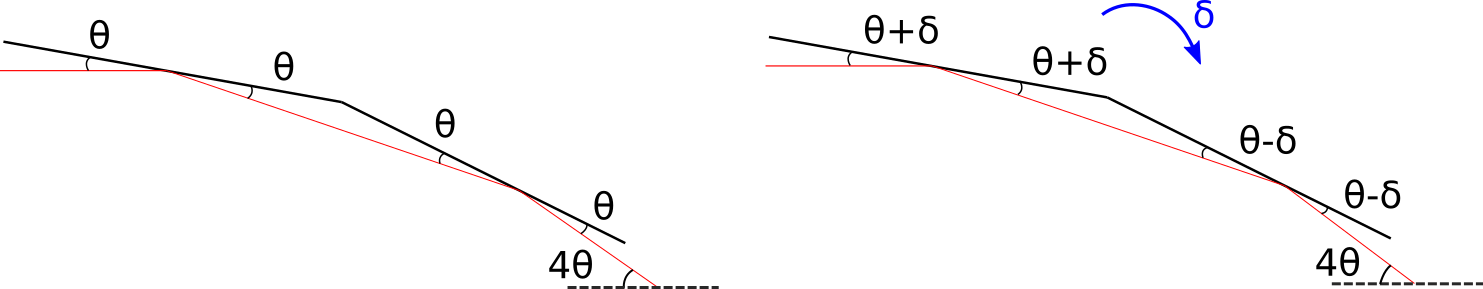
\includegraphics[width=10cm]{wolter_robustness.png}
\caption{2回反射による設置角度誤差のキャンセル}
\label{fig:wolter_robustness}
\end{figure}

このことは、2回反射が設置角度誤差に対して安定した結像性能を持つことの大きな理由である。
また、Wolter I型ミラーは近似的にアッベの正弦条件を満たす。
無限遠の光源に対するアッベの正弦条件は図\ref{fig:abbe_sine_condition_for_parallel_light}の変数について
\[
    h = f \sin u
\]
と表される。


\begin{figure}[b]
\centering
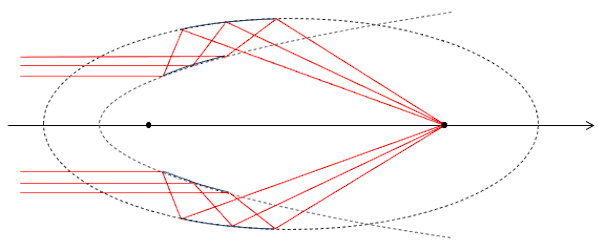
\includegraphics[width=10cm]{wolter_type_3.png}
\caption{無限遠の光源に対するアッベの正弦条件}
\label{fig:abbe_sine_condition_for_parallel_light}
\end{figure}

アッベの正弦条件を満たすとき、光軸に対して角度がついた平行光に対して球面収差とコマ収差のない結像系であると言える。

2回反射を利用した集光ミラーであって、全周にわたって回転したものをWolterミラーという。
2回の反射面は、放物線、双曲線、楕円の3種類の2次曲線を組み合わせた図形の回転体として与えられる。
焦点を共有するように設計・配置することで1点に集光する系を構成することができる。
WolterミラーにはI型(図\ref{fig:wolter_type_1})、II型(図\ref{fig:wolter_type_2})、III型(図\ref{fig:wolter_type_3})の3種類が存在する。
I型は放物面、双曲面の順に反射する。
いずれも内面で反射する形状になっているため、\ref{chap1_wolter_fabrication_process}節で述べるマンドレル転写加工がしやすく高精度な作製が期待できる。
また、受光面積を広げるため、\ref{chap1_nested_wolter_mirror}節で述べるような複数枚のネスト構造を構成することが比較的容易である。
II型は放物面内面、双曲面外面の順に反射する構成になっている。
I型に比べ加工・設置が難しくなるが、2枚が覆いかぶさるように重ねた配置にすることができ、焦点距離を短くし光学系全体を小型化することができる。
III型も同様に加工・設置が難しくなるが、焦点距離を短くするような配置が可能になる。
II型、III型は凸面形状ミラーの加工の困難さからWolterミラーとしては実用化されていない。
KB型配置ではIII型に対応する構成での集光光学系が提案されている。\cite{Yamada:20}

\begin{figure}[b]
\centering
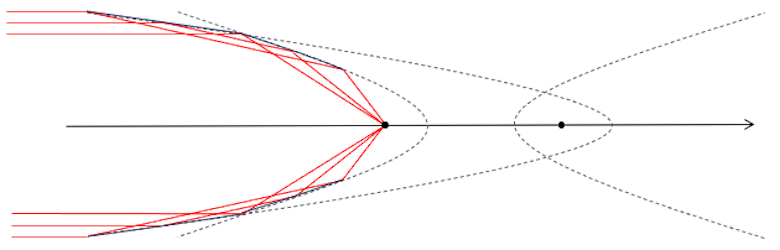
\includegraphics[width=10cm]{wolter_type_1.png}
\caption{Wolter I型}
\label{fig:wolter_type_1}
\end{figure}

\begin{figure}[b]
\centering
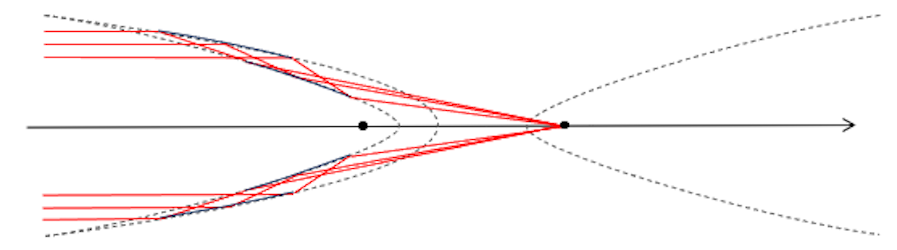
\includegraphics[width=10cm]{wolter_type_2.png}
\caption{Wolter II型}
\label{fig:wolter_type_2}
\end{figure}

\begin{figure}[b]
\centering
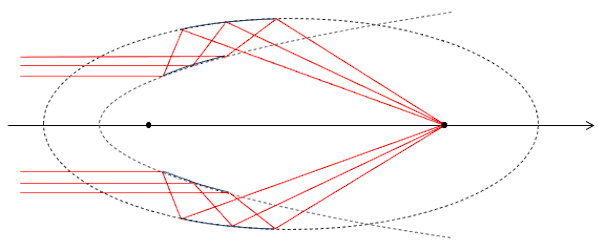
\includegraphics[width=10cm]{wolter_type_3.png}
\caption{Wolter III型}
\label{fig:wolter_type_3}
\end{figure}

\subsection{ネスト型Wolterミラー}
\label{chap1_nested_wolter_mirror}

Wolterミラーのような円筒形のミラー、特にX線を反射するため斜入射角が小さく設計されたミラーにおいて、中空になっている内側部分を通過する光を集めることができず、集光強度を高める上で不都合である。
これを解決する方法として、図\ref{fig:nested_wolter_mirror}のように口径の異なるWolterミラーを内側に挿入するというものがある。\cite{BuitragoCasas2017}

\begin{figure}[b]
\centering
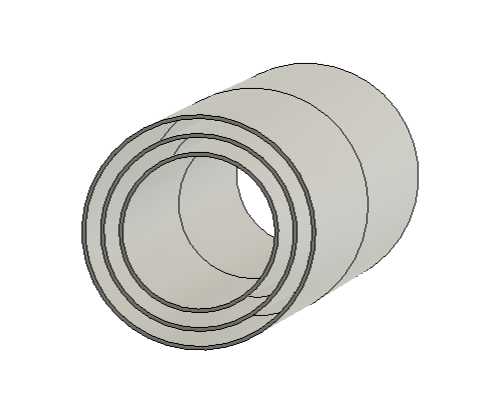
\includegraphics[width=8cm]{nested_wolter_mirror.png}
\caption{Nested Wolterミラーの例}
\label{fig:nested_wolter_mirror}
\end{figure}

このようにネスト構造にすることで、受光面積を大きくすることができ、集光強度を上げることができる。
このようなネスト構造を構成できるのはI型のみであり、その点で天体応用としてはI型が有力な選択肢となる。
実際、FOXSI3でもI型をネストしたNested Wolterミラーが搭載されていた。
このように受光面積の観点では非常に有利であるNested Wolterミラーだが、ネストする枚数を増やすほどその設置が困難になるという問題がある。
ミラー同士の角度・光軸のずれなど、調整しなければならない誤差要因が増えるためである。
そのため、ネストの構成後に光学系を統合的に計測する方法が必要になる。
また、ミラー同士をネストさせたあとにプローブを挿入して計測することは困難であるため、その統合的な評価は間接測定によって行われなければならない。

\newpage
\section{FOXSI4におけるWolterミラー}
\label{chap1_background}

\subsection{FOXSI4}
\label{chap1_foxsi}

2018年に打ち上げられたFOXSI3では太陽コロナのX線写真を撮影することに成功した。\cite{weko_20796_1}
図\ref{fig:foxsi-fullsun-image}はその撮影像の1枚である。
FOXSI3よりも高い分解能で太陽コロナの像を撮影することを目標として、光学系をアップデートしたFOXSI4が2023年頃の打ち上げを予定している。\cite{2019AGUFMSH31C3315V}
ここで搭載されるWolterミラーについて、作製精度を

\begin{figure}[h]
\centering
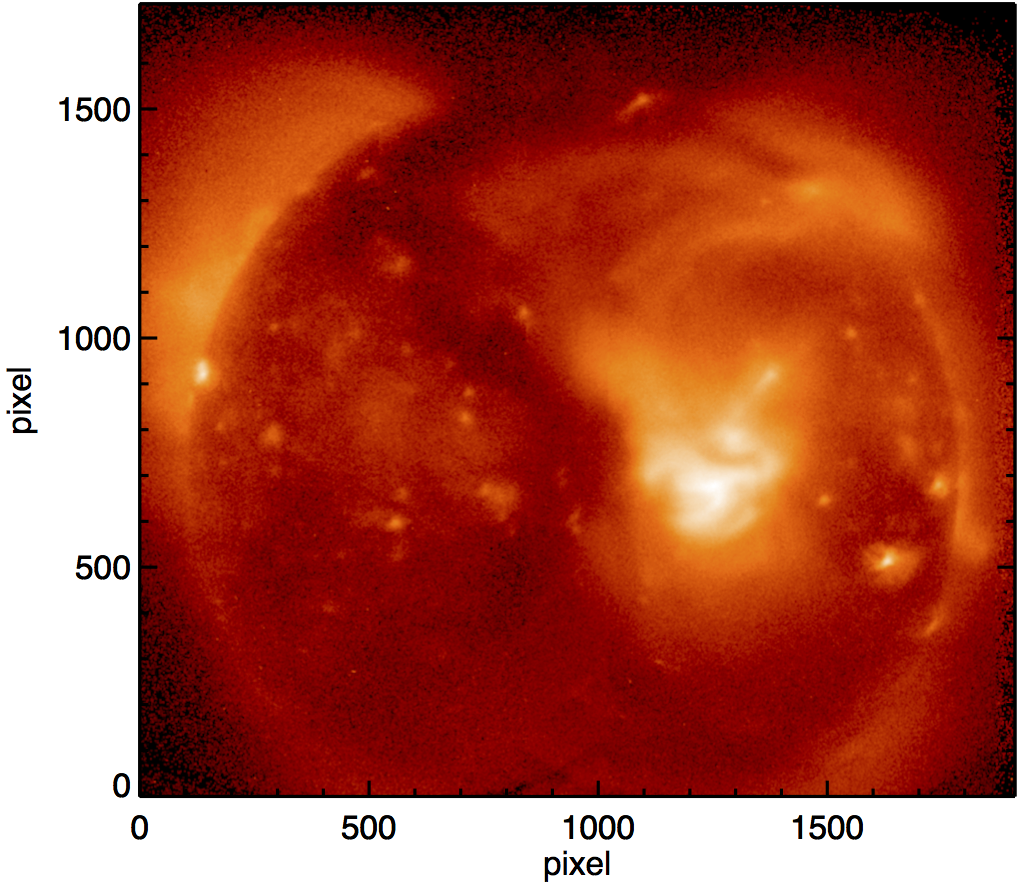
\includegraphics[width=6cm]{foxsi3-full-sun.png}
\caption{FOXSI-3 phoenix full sun soft X-ray image \cite{weko_20796_1}}
\label{fig:foxsi-fullsun-image}
\end{figure}

\subsection{Wolterミラーの設計}
\label{chap1_wolter_arrangement}
FOXSI4に搭載予定のX線用Wolterミラーは、放物面、双曲面の順に反射するI型に分類される。

以下では、開発対象となっているWolter I型のミラーの設計パラメータを図\ref{fig:wolter_params}に対応して表\ref{tb:wolter_params}に示す。

\begin{figure}[h!]
\centering
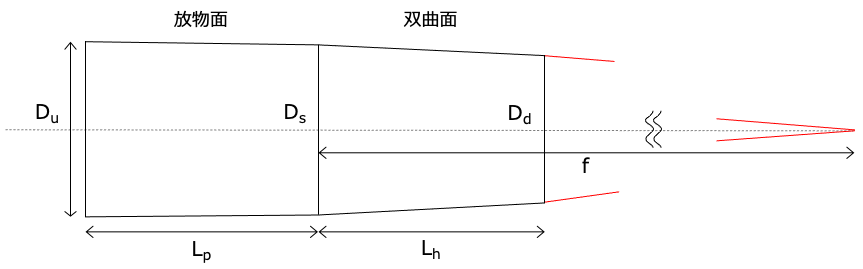
\includegraphics[width=12cm]{wolter_mirror_params.png}
\caption{Wolterミラーの設計変数}
\label{fig:wolter_params}
\end{figure}

\begin{table}[ht]
\begin{center}
  \begin{tabular}{|c|c|l|} \hline
    変数 & 値 & 説明 \\ \hline
    $d_u$ & 60.801 mm & 上流端開口直径 \\
    $d_s$ & 60.000 mm & 接合部直径 \\
    $d_d$ & 57.689 mm & 下流端開口直径 \\
    $l_p$ & 102.501 mm & 放物面部長さ \\
    $l_h$ & 97.499 mm & 双曲面部長さ \\
    $ml$ & 200.000 mm & ミラー全長 \\
    $f$ & 2000.000 mm & 焦点距離 \\ \hline
  \end{tabular}
  \caption{Wolterミラー各設計変数の値}
  \label{tb:wolter_params}
\end{center}
\end{table}

これらを図\ref{fig:wolter_profile}のように放物面部および双曲面部の設計半径として表すと、下式(パラメータは図\ref{tb:wolter_profile_constants})のようになる。
$f1$は座標系の平行移動に関して任意であるため、変数として表記する。

\begin{equation}
    r_p(z) = \sqrt{ -4p(z - p - f_2) } \\
\end{equation}

\begin{equation}
    r_h(z) = b \sqrt{ \frac{(z - (f_1 + f2) / 2)^2}{a^2} - 1.0 }
\end{equation}

\begin{figure}[h]
\centering
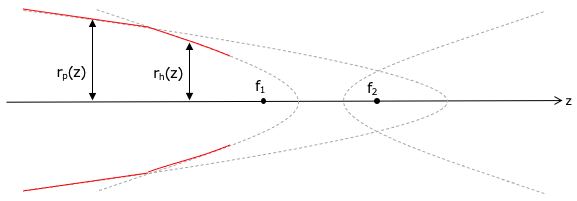
\includegraphics[width=10cm]{mirror_profile.png}
\caption{Wolterミラーの設計半径}
\label{fig:wolter_profile}
\end{figure}

\begin{table}[htb]
    \begin{center}
      \begin{tabular}{|c|c|l|} \hline
        定数 & 値 & 説明 \\ \hline
        $p$ & 0.0562 mm & 下流端開口直径 \\
        $a$ & 1000.056 mm & 放物面部長さ \\
        $b$ & 10.606 mm & 双曲面部長さ \\ 
        $f_1$ & 任意 & 焦点座標 \\
        $f_2$ & $f_1 + 2 \sqrt{ a^2 + b^2 }$  & 共焦点座標 (双曲線のもう一方の焦点) \\\hline
      \end{tabular}
      \caption{Wolterミラーの設計半径における定数}
      \label{tb:wolter_profile_constants}
    \end{center}
\end{table}


\subsection{マンドレル電鋳法}
\label{chap1_mirror_mandrel}

ここで、測定対象となるWolterミラーの製造プロセスについて述べる。
凹状になっている回転体形状のミラー内面を高精度に加工することは難しく、凸形状のマンドレルを高精度に加工し、これに対してさらに転写加工を行うという手法が提案されている。\cite{Mimura2018}
図\ref{fig:mandrel_plating_pictures}に回転楕円ミラーに対するマンドレル電鋳法の一連の流れを示す。

\begin{figure}[!ht]
\centering
\subfloat[高精度に加工されたマンドレル]{
    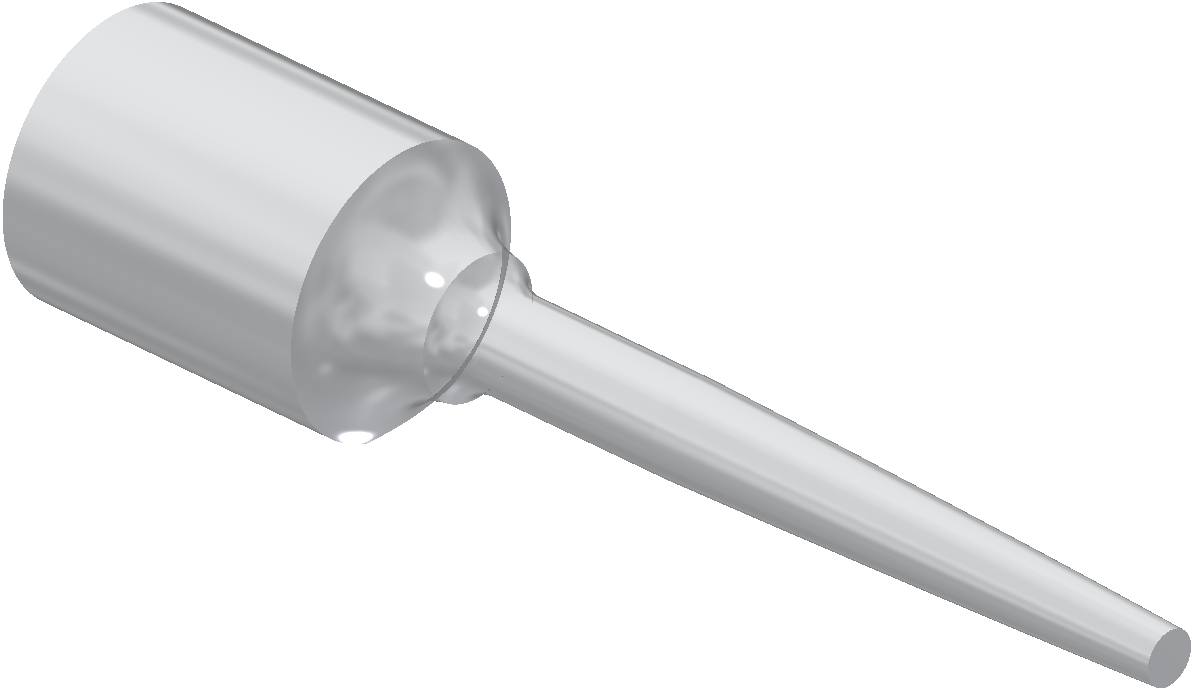
\includegraphics[width=4cm]{mandrel_before_plating.png}
    \label{fig:mandrel_before_plating}
}
\subfloat[マンドレルに転写されたミラー]{
    \centering
    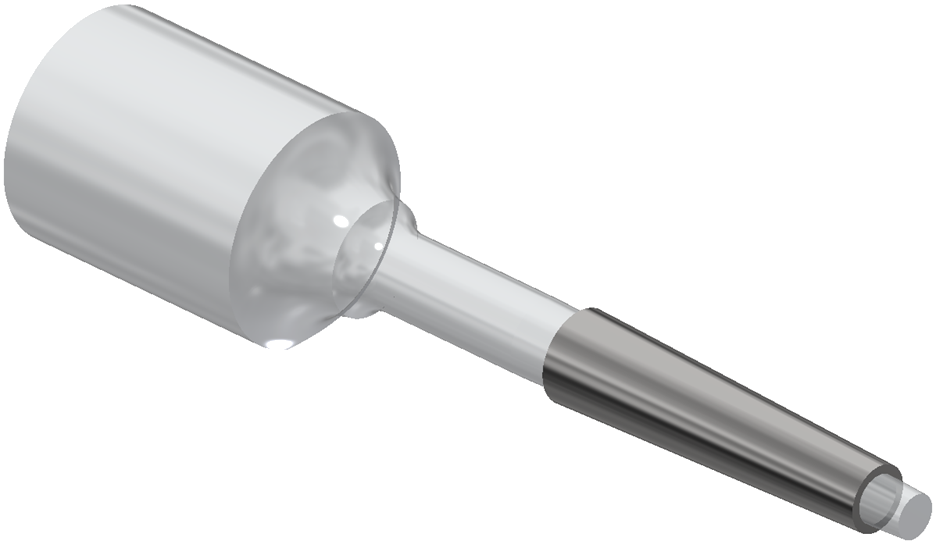
\includegraphics[width=4cm]{mandrel_after_plating.png}
    \label{fig:mandrel_after_plating}
}
\subfloat[取り外されたミラー]{
    \centering
    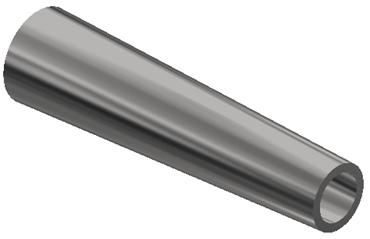
\includegraphics[width=4cm]{detached_mirror.png}
    \label{fig:detached_mirror}
}
\caption[]{マンドレル電鋳法の模式図}
\label{fig:mandrel_plating_pictures}
\end{figure}

3種類のWolterミラーのうち、2回の反射が内面において起こるI型では、同様の手法で加工が可能であり、既にこの方法で真円度誤差\SI{20}{\micro \metre}程度以下の精度でWolterミラーが作製されている。\cite{Egawa2019}

\subsection{直接計測法}
\label{chap1_direct_measurement}

久米らは、図\ref{fig:profile_measurement_schematic}および図\ref{profile_measurement}に示すように、接触式変位計を用いて周方向形状誤差プロファイルおよび長手方向形状誤差プロファイルを数本ずつ取得し、さらにこれらを組み合わせることで3次元形状を決定するという方法を提案した。\cite{Kume2017}
しかしこれらの誤差プロファイル計測手法では、ある始点からの変位量しか測定できず、直径や長手プロファイルの傾き(テーパー角)の情報を取得することができない。
このような誤差プロファイル計測では得られない情報を補完する計測方法が必要である。
また、高精度に加工されたミラー内面に接触式のプロファイル計測を適用することは、その表面形状を悪化させる恐れがある。
そのため、非接触式の計測方法を用いることが望ましい。

\begin{figure}[h]
\centering
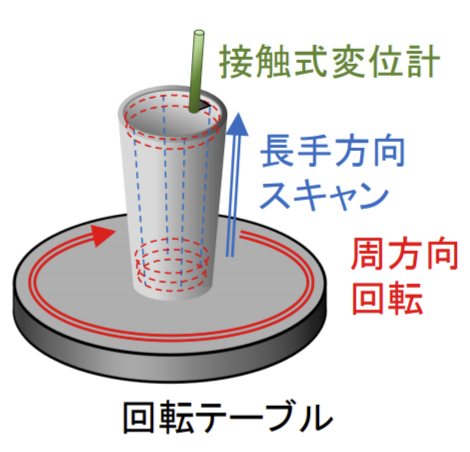
\includegraphics[width=5cm]{profile_measurement_schematic.png}
\caption{接触式誤差プロファイル計測}
\label{fig:profile_measurement_schematic}
\end{figure}

\begin{figure}[!ht]
\centering
\subfloat[長手方向形状誤差プロファイル]{
    \centering
    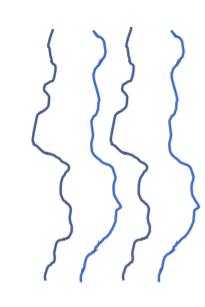
\includegraphics[height=4cm]{meridional_profile.png}
    \label{fig:meridional_profile}
}
\subfloat[周方向形状誤差プロファイル]{
    \centering
    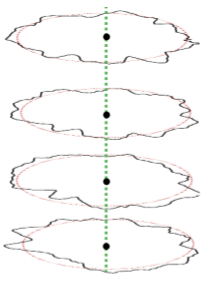
\includegraphics[height=4cm]{sagital_profile.png}
    \label{fig:sagital_profile}
}
\subfloat[3次元形状誤差プロファイル]{
    \centering
    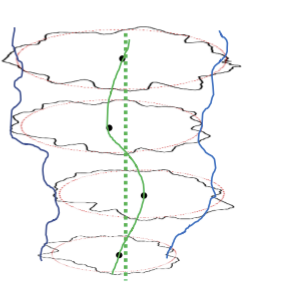
\includegraphics[height=4cm]{combined_profile.png}
    \label{fig:combined_profile}
}
\caption[]{プロファイル計測による3次元プロファイルの構成}
\label{fig:profile_measurement}
\end{figure}



\clearpage
% -------------------------------------------------- %
% section
% -------------------------------------------------- %
\newpage
\section{波面計測法によるミラー形状の解析}
\label{chap1_wave_metrics}

プロファイル計測では得られない情報を取得すること、またネスト構造のミラーを計測可能な間接測定であることという2つの要請を満足させる方法として、波動光学の理論を応用した波面計測法がある。
波動光学では、光波を複素スカラー場$U(P)=A(P)\exp(i\Phi(P))$とし、等位相面$\Phi(P)=const$を波面とよぶ。
一般に、ある光が1点に収束するとき、光の波面は収束点を中心とする球面になる。
もし仮にミラーが入射光を完全に1点に集めるとすると、ミラーの出口、下流端開口に現れる光波は球面波になるはずだが、現実にはミラーの設計の特徴や加工時の誤差を反映して波面が変形する。
波面計測法とは、この波面のずれを波面誤差$\Delta\Phi(P)/k$(長さの次元を持つ)として求め、波面誤差からその原因となる誤差の量を算出するという計測方法である。
可視光光源に対する波面の計測手法として広く利用されているのが、シャックハルトマンセンサーである。
シャックハルトマンセンサーすごいよね
しかし、非常に細い輪帯とシャックハルトマンセンサーは相性が悪く


\clearpage
% -------------------------------------------------- %
% section
% -------------------------------------------------- %
\newpage

\section{本研究で測定対象となるWolterミラー}
\label{chap1_target_wolter}

\subsection{天文用X線Wolterミラーの持つ特性}
\label{chap1_wolter_specific_feature}

口径が大きく、X線に対応するため射入射角を小さく設定したWolterミラーはNAがやや小さくなり、波面計測において求めなければならない波面は図\ref{fig:wolter_thinring}に示すように非常に細い輪帯状になる。
輪帯の幅(外円と内円の半径の差)は実に\SI{363.3}{\micro \metre}であり、波面計測に求められる空間分解能は非常に高いものとなる。
半径方向の位相分布を見る際、極値を取っている状態を判別するには、少なくとも3ピクセルに分割できている必要があり、\SI{100}{\micro \metre}程度の空間分解能で計測できなければならない。
波面精度を十分に確保しつつ、空間分解能が十分に高い波面計測法を開発する必要がある。

\begin{figure}[h!]
\centering
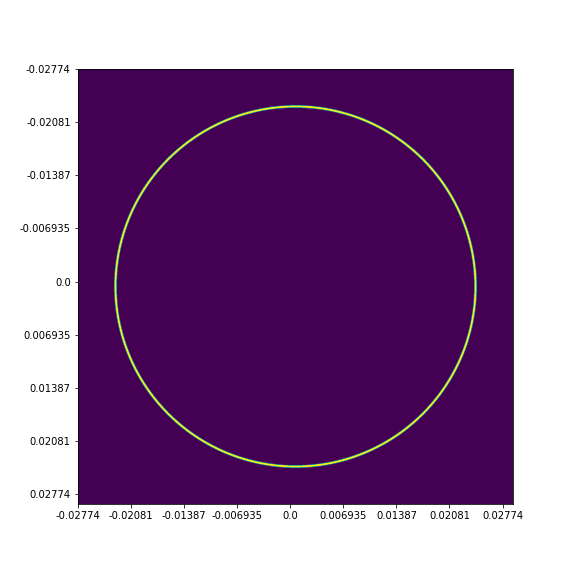
\includegraphics[width=7cm]{wolter_thinring.png}
\caption{Wolterミラー下流端面における集光波面}
\label{fig:wolter_thinring}
\end{figure}


\clearpage
% -------------------------------------------------- %
% section
% -------------------------------------------------- %
\newpage
\section{本論文の目的}
\label{chap1_purpose}

JAXAの進めるミッションLynxでは、0.5秒角分解能の望遠鏡の搭載を大きな目標として掲げている。\cite{Gaskin2019}
これに先立って、2023年に打ち上げられるFOXSI4に搭載するWolterミラーの加工について、1秒角分解能を目標として設定する。
これを実現する上で問題となる加工誤差はどのようなものであるかを統合的な計測から測定し、加工プロセスへ直ちにフィードバックするための系を開発することが、本研究の目的となる。

% -------------------------------------------------- %
% section
% -------------------------------------------------- %
\section{本論文の構成}
\label{chap1_outline}

\ref{chap2}章では、測定対象のWolterミラーに対して様々な種類の誤差を与え、その際の集光波面の変化をシミュレーションする。
この集光波面の強度分布から、目標とする1秒角分解能の達成に際して要求される許容誤差の範囲を見積もるとともに、\ref{chap3}章以降で扱う波面計測法における解析に用いる基底を前もって解析しておく。
\ref{chap3}章では、波面計測における様々な手法の中でWolterミラーの計測に適した方法を検討するため、シミュレーションによってその利点・欠点を洗い出し、最終的に計測に用いる方法を決定する。
\ref{chap4}章では、\ref{chap3}章で提案された手法について、ミラーに比べ加工誤差が小さく、より理想的な集光が期待できるレンズを用いて、その正当性を実証する。
\ref{chap5}章では、実際に加工された3枚の天文用Wolterミラーに対して計測実験を行い、\ref{chap2}でシミュレーションによって求めた誤差応答との比較からミラー内部形状の誤差に関する解析を行う。
最後に、\ref{chap6}章で考察、結論および今後の展望について述べる。

%%%%%%%%%%%%%%%%%%%%%%%%%%%%%%%%%%%%%%%%%%%%%%%%%%%%%%%%%%%%%%%%%%%%%%%%%%%%%
%%% Local Variables:
%%% mode: katex
%%% TeX-master: "../thesis"
%%% End:
